\documentclass{book}
\usepackage[spanish]{babel}
\usepackage[utf8]{inputenc}
\usepackage{graphicx}

\title{Reporte de análisis}
%%
%% Escriban el nombre de los colaboradores aquí
%%
\author{-}

\begin{document}

\maketitle

\chapter{Análisis}
El programa deberá convertir una Expresión Regular (E.R.) a un Autómata Finito Determinista(A.F.D.). 
Dicha tarea se programará apegándose al algoritmo <<del Árbol>>.


\section{El algoritmo}

La entrada del algoritmo es: una expresión regular, la salida del algoritmo es: un A.F.D.
Los pasos del algoritmo se pueden listar como:

\begin{enumerate}
\item Extender la E.R. que se va a convertir.
\item Construir el árbol de análisis sintáctico correspondiente a la E.R.
\item Anotar las posiciones de los símbolos que están en la E.R.
\item Anotar en cada nodo si es anulable o no.
\item Anotar en cada nodo las posiciones de la función primero().
\item Anotar en cada nodo las posiciones de la función último().
\item Llenar la tabla de las posiciones siguientes.
\item Determintar los estados del A.F.D usando los siguientes.
\item Marcar el estado inicial y los finales.
\end{enumerate}

En la tabla \ref{fig:tabla1} se puede ver ....
\begin{figure}
\centering
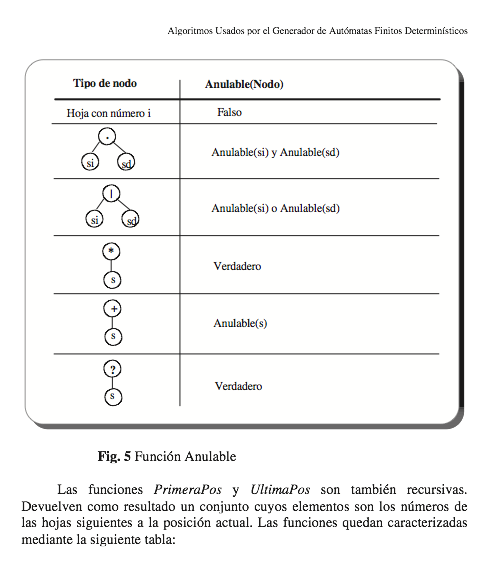
\includegraphics[width=12cm]{img/tabla1.png}
\caption{Tabla de ...}
\label{fig:tabla1}
\end{figure}

En la tabla \ref{fig:tabla2} se puede ver ....
\begin{figure}
\centering
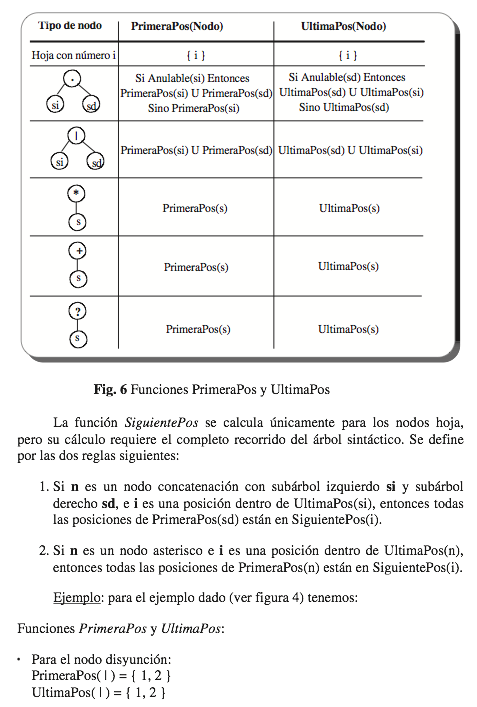
\includegraphics[width=12cm]{img/tabla2.png}
\caption{Tabla de ...}
\label{fig:tabla2}
\end{figure}

En la tabla \ref{fig:tabla3} se puede ver ....
\begin{figure}
\centering
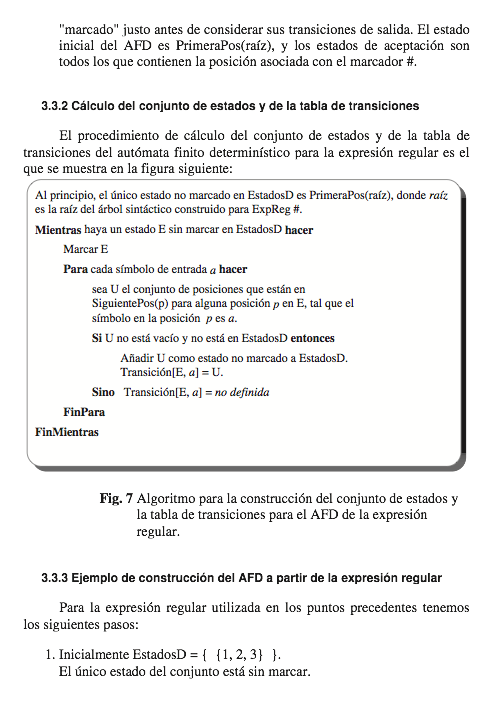
\includegraphics[width=12cm]{img/tabla3.png}
\caption{Tabla de ...}
\label{fig:tabla3}
\end{figure}

\end{document}
